%
%  untitled
%
%  Created by Dean Freestone on 2012-10-09.
%  Copyright (c) 2012 . All rights reserved.
%
\documentclass[]{article}

\usepackage{color}                    % For creating coloured text and background
\newcommand{\dean}[1]{\textcolor{green}{#1}}

% Use utf-8 encoding for foreign characters
\usepackage[utf8]{inputenc}

% Setup for fullpage use
\usepackage{fullpage}

% Uncomment some of the following if you use the features
%
% Running Headers and footers
%\usepackage{fancyhdr}

% Multipart figures
\usepackage{subfigure}

% More symbols
\usepackage{amsmath}
\usepackage{amssymb}
\usepackage{latexsym}

% Surround parts of graphics with box
\usepackage{boxedminipage}

% Package for including code in the document
\usepackage{listings}

% If you want to generate a toc for each chapter (use with book)
\usepackage{minitoc}

% This is now the recommended way for checking for PDFLaTeX:
\usepackage{ifpdf}

%\newif\ifpdf
%\ifx\pdfoutput\undefined
%\pdffalse % we are not running PDFLaTeX
%\else
%\pdfoutput=1 % we are running PDFLaTeX
%\pdftrue
%\fi

\ifpdf
\usepackage[pdftex]{graphicx}
\else
\usepackage{graphicx}
\fi
\title{A New Kalman Filter for Sigmoidal Nonlinearities}
\author{Dean R. Freestone, Parham Aram, David B. Grayden, Dragan Nesic, ....  }

\date{2012-10-09}

\begin{document}

\ifpdf
\DeclareGraphicsExtensions{.pdf, .jpg, .tif}
\else
\DeclareGraphicsExtensions{.eps, .jpg}
\fi

\maketitle


\begin{abstract}
\end{abstract}

\section{Introduction}

\begin{figure}[!ht]
	\centering
		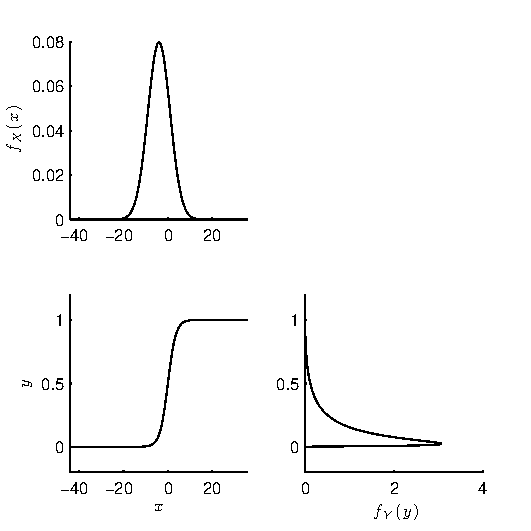
\includegraphics[scale=1]{./Figures/pdf/Mapping.pdf}
	\caption{\textbf{Transformation of a Gaussian through a sigmoid.}}
	\label{fig:label}
\end{figure}
\begin{figure}[!ht]
	\centering
		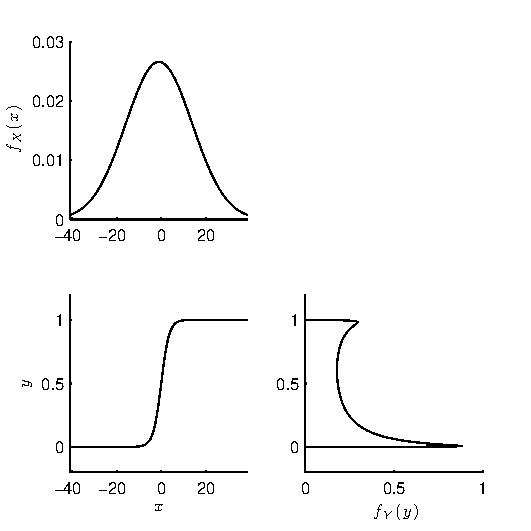
\includegraphics[scale=1]{./Figures/pdf/Mapping2.pdf}
	\caption{\textbf{Transformation of a Gaussian through a sigmoid.}}
	\label{fig:label}
\end{figure}

\subsection{Expected Value of a Gaussian Transformed by an Error Function Sigmoid}
Let's look at the transformation of a Gaussian random variable through a typical sigmoidal function. Let our Gaussian RV be described by the probability density function
\begin{equation}\label{eq:Gaussian_pdf}
	f_X(x) = \frac{1}{\sigma_x\sqrt{2\pi}}\exp\left(-\frac{(x-\bar{x})^2}{2\sigma_x^2}\right).
\end{equation}

An alternate form of the sigmoid function than the one that is typically used is
\begin{align}
	g(v) &= \frac{1}{\sqrt{2\pi}\varsigma}\int_{-\infty}^{v}\exp\left(-\frac{(z-v_0)^2}{2\varsigma^2}\right)\,\mathrm{d}z \\
	&= \frac{1}{2}\left(\mathrm{erf}\left(\frac{v-v_0}{\varsigma\sqrt{2}}\right) + 1\right).
\end{align}
\begin{figure}[ht!]
	\centering
		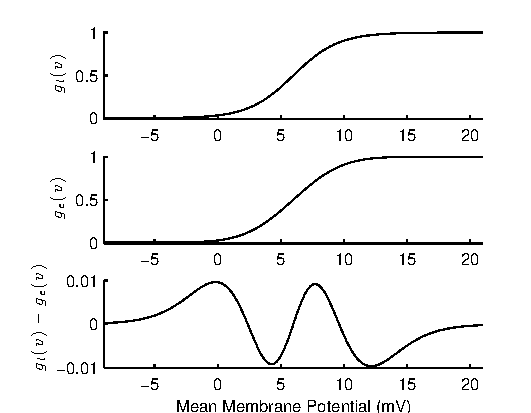
\includegraphics[scale=1]{./Figures/pdf/DifferentSigmoids.pdf}
	\caption{caption}
	\label{fig:label}
\end{figure}

Now we consider the mapping of the GRV (defined in equation~\ref{eq:Gaussian_pdf}) through this new sigmoid. In a similar vein as before, we will first consider a simple case where $v_0 = 0$ and $\varsigma = 1$. So we have
\begin{align}
	Y &= g(X) \\
	&= \frac{1}{\sqrt{2\pi}}\int_{-\infty}^{x}\exp\left(-\frac{z^2}{2}\right)\,\mathrm{d}z \\
	&= \frac{1}{2}\left(\mathrm{erf}\left(\frac{x}{\sqrt{2}}\right) + 1\right)
\end{align}
and
\begin{align}
	f_Y(y) &= |h'(y)|f_X[h(y)] \\
	&= \frac{h'(y)}{\sigma_x\sqrt{2\pi}}\exp\left(-\frac{(h(y)-\bar{x})^2}{2\sigma_x^2}\right)
\end{align}
where
\begin{equation}
	h(y) = g^{-1}(Y).
\end{equation}
As before, we have the expected value of the transformed Gaussian as
\begin{align}
	\mathbb{E}(y) &= \int_{-\infty}^{\infty}yf_Y(y) \,\mathrm{d}y \\
	&=\int_{-\infty}^{\infty}\frac{y h'(y)}{\sigma_x\sqrt{2\pi}}\exp\left(-\frac{(h(y)-\bar{x})^2}{2\sigma_x^2}\right)\,\mathrm{d}y. \label{eq:expected_value_erf_sigmoid}
\end{align}

Now the papers by Brenden J. Frey (Variational inference for continuous sigmoidal Bayesian networks, 1999 and Variational learning in nonlinear Gaussian belief networks, Neural Computation 1999) provide a closed-form solution to the expectation. This solution is
\begin{align}
	\mathbb{E}(y) &= g\left(\frac{\bar{x}}{\sqrt{1+\sigma^2}}\right) \\
	&= \frac{1}{2}\left(\mathrm{erf}\left(\frac{\bar{x}}{\sqrt{2}\sqrt{1+\sigma^2}}\right)+1\right).
\end{align}
This is shown in Figure~\ref{fig:MappingThroughERF}, where the a Monte-Carlo simulation was used to test the analytic result. The predicted expected value and the actual numerical expected value correspond nicely.
\begin{figure}[!ht]
	\centering
		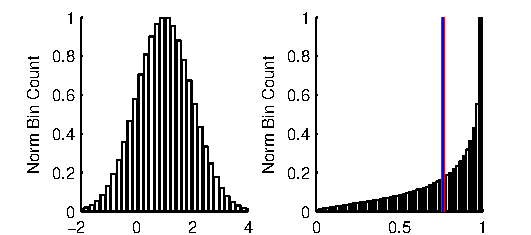
\includegraphics[scale=1]{./Figures/pdf/MappingThroughERF.pdf}
	\caption{\textbf{Monte Carlo simulation result confirming the analytic solution.}}
	\label{fig:MappingThroughERF}
\end{figure}

The derivation proceeds as follows. The expected value is defined by
\begin{align}
\mathbb{E}\left[y\right] =& \int_{-\infty}^{\infty}g(x)f_X(x)\,\mathrm{d}x \\
	&=\frac{1}{\sqrt{2\pi}}\int_{-\infty}^{\infty}\int_{-\infty}^{x}\exp\left(-\frac{z^2}{2}\right)f_X(x)\,\mathrm{d}z\,\mathrm{d}x.
\end{align}
Now we can make the substitution $z=w-x$ to get $x$ out of the integral terminal giving
\begin{align}
\mathbb{E}\left[y\right] &=\frac{1}{\sqrt{2\pi}} \int_{-\infty}^{\infty} \int_{-\infty}^{0} \exp\left(-\frac{\left(w-x\right)^2}{2}\right)f_X(x) \, \mathrm{d}w\,\mathrm{d}x.
\end{align}
The order of integration can be changed without changing the limits of integration giving
\begin{align}
\mathbb{E}\left[y\right]  &= \frac{1}{\sqrt{2\pi}} \int_{-\infty}^{0} \int_{-\infty}^{\infty} \exp\left(-\frac{\left(w-x\right)^2}{2}\right)f_X(x) \, \mathrm{d}x\,\mathrm{d}w \\	
&=\frac{1}{2\pi\sigma}\int_{-\infty}^{0}\int_{-\infty}^{\infty}\exp\left(-\frac{\left(w-x\right)^2}{2}\right)\exp\left(-\frac{(x-\mu)^2}{2\sigma^2}\right)\,\mathrm{d}x\,\mathrm{d}w \\
&=\frac{1}{2\pi\sigma}\int_{-\infty}^{0}\int_{-\infty}^{\infty}\exp\left(-\frac{\left(w-x\right)^2}{2}-\frac{(x-\mu)^2}{2\sigma^2}\right)\,\mathrm{d}x\,\mathrm{d}w
\end{align}
\dean{From Wolfram Alpha, our target solution is
\begin{equation}
	\int_{-\infty}^{\infty}\exp\left(-\frac{\left(w-x\right)^2}{2}-\frac{(x-\mu)^2}{2\sigma^2}\right)\,\mathrm{d}x = \frac{\sqrt{2\pi}\sigma}{\sqrt{\sigma^2+1}}\exp\left(-\frac{\left(w-\mu\right)^2}{2\left(\sigma^2+1\right)}\right),
\end{equation}
which leads to 
\begin{equation}
	\mathbb{E}\left[y\right] = \frac{1}{2\pi}\frac{\sqrt{2\pi}}{\sqrt{\sigma^2+1}} \int_{-\infty}^{0}\exp\left(-\frac{\left(w-\mu\right)^2}{2\left(\sigma^2+1\right)}\right)
\end{equation}}
Now we need to integrate out $x$, so we collect all the $x$-related terms
\begin{align}
\mathbb{E}\left[y\right] &= \frac{1}{2\pi\sigma} \int_{-\infty}^{0} \int_{-\infty}^{\infty} \exp\left(-\frac{1}{2}\left(w^2-2wx+x^2\right)-\frac{1}{2\sigma^2}\left(x^2-2\mu x + \mu^2\right)\right) \,\mathrm{d}x \,\mathrm{d}w \\
&=\frac{1}{2\pi\sigma}\int_{-\infty}^{0}\int_{-\infty}^{\infty}\exp\left(-\frac{1}{2\sigma^2}\left(\sigma^2w^2-\sigma^22wx+\sigma^2x^2 + x^2-2\mu x + \mu^2\right)\right)\,\mathrm{d}x\,\mathrm{d}w \\
&=\frac{1}{2\pi\sigma}\int_{-\infty}^{0}\int_{-\infty}^{\infty}\exp\left(-\frac{1}{2\sigma^2}\left(\left(\sigma^2 +1\right)x^2 - 2\mu x - \sigma^22w x + \sigma^2w^2 +  \mu^2\right)\right)\,\mathrm{d}x\,\mathrm{d}w \\
&=\frac{1}{2\pi\sigma}\int_{-\infty}^{0}\exp\left(-\frac{1}{2\sigma^2}\left(\sigma^2w^2 +  \mu^2\right)\right)\int_{-\infty}^{\infty}\exp\left(-\frac{\sigma^2 +1}{2\sigma^2}x^2 + \frac{\sigma^2w+\mu}{\sigma^2}x\right)\,\mathrm{d}x\,\mathrm{d}w \\
\end{align}

Now we integrate out $x$. Let
\begin{align}
	\int_{-\infty}^{\infty}\exp\left(-\frac{\sigma^2 +1}{2\sigma^2}x^2 + \frac{\sigma^2w+\mu}{\sigma^2}x\right)\,\mathrm{d}x =& \int_{-\infty}^{\infty}\exp\left(ax^2+bx\right)\,\mathrm{d}x \\
	=& \int_{-\infty}^{\infty}\exp\left(a\left(x+\frac{b}{2a}\right)^2 + \frac{b^2}{4a} \right)\,\mathrm{d}x \\
	=& \exp\left(- \frac{b^2}{4a}\right)\int_{-\infty}^{\infty}\exp\left(\frac{\left(x+\frac{b}{2a}\right)^2}{a^{-1}}  \right)\,\mathrm{d}x \\
	=& \exp\left(- \frac{b^2}{4a}\right)\frac{1}{\sqrt{-a}}\int_{-\infty}^{\infty}\exp\left(-c^2\right)\,\mathrm{d}c \\
	=& \frac{\sqrt{\pi}}{\sqrt{-a}}\exp\left(-\frac{b^2}{4a}\right),
\end{align}
where
\begin{align}
	a =& -\frac{\sigma^2 + 1}{2\sigma^2} \\
	b =& \frac{\sigma^2w + \mu}{\sigma^2} \\
	c =& \frac{x+\frac{b}{2a}}{\sqrt{-a^{-1}}} \\
	\frac{\mathrm{d}c}{\mathrm{d}x} =& \frac{1}{\sqrt{-a^{-1}}} \\
	\mathrm{d}x =& \mathrm{d}c \sqrt{-a^{-1}}.
\end{align}
Now substituting back to replace $a$ and $b$ we get
\begin{align}
	\frac{\sqrt{\pi}}{\sqrt{-a}}\exp\left(-\frac{b^2}{4a}\right) =& \frac{\sqrt{\pi}}{\sqrt{\frac{\sigma^2 + 1}{2\sigma^2}}}\exp\left(\frac{\left(\frac{\sigma^2w + \mu}{\sigma^2}\right)^2}{\frac{4(\sigma^2 + 1)}{2\sigma^2}}\right) \\
	=& \frac{\sqrt{2\pi}\sigma}{\sqrt{\sigma^2 + 1}}\exp\left(\frac{\sigma^2}{2(\sigma^2 + 1)}\left(\frac{\sigma^2w + \mu}{\sigma^2}\right)^2\right) \\
	=& \frac{\sqrt{2\pi}\sigma}{\sqrt{\sigma^2 + 1}}\exp\left(\frac{\left(\sigma^2w + \mu\right)^2}{2\sigma^2(\sigma^2 + 1)}\right) \\
\end{align}
Now putting it back together again \dean{(this agrees with Wolfram Alpha)} we get
\begin{align}
\mathbb{E}\left[y\right] &=\frac{1}{2\pi\sigma} \int_{-\infty}^{0} \exp\left(-\frac{1}{2\sigma^2} \left(\sigma^2w^2 +  \mu^2\right)\right)\frac{\sqrt{2\pi}\sigma}{\sqrt{\sigma^2+1}}\exp\left(\frac{\left(\mu + \sigma^2 w\right)^2}{2\sigma^2\left(\sigma^2 + 1\right)}\right) \,\mathrm{d}w \\
&=\frac{1}{2\pi\sigma}\frac{\sqrt{2\pi}\sigma}{\sqrt{\sigma^2+1}}\int_{-\infty}^{0} \exp\left(-\frac{1}{2\sigma^2}\left(\sigma^2w^2 +  \mu^2\right)\right)\exp\left(\frac{\left(\mu + \sigma^2w\right)^2}{2\sigma^2\left(\sigma^2+1\right)}\right) \,\mathrm{d}w \\
&=\frac{1}{2\pi}\frac{\sqrt{2\pi}}{\sqrt{\sigma^2+1}}\int_{-\infty}^{0} \exp\left(-\frac{\left(\sigma^2+1\right)\left(\sigma^2w^2 +  \mu^2\right)}{2\sigma^2\left(\sigma^2+1\right)}+\frac{\left(\mu+\sigma^2w\right)^2}{2\sigma^2\left(\sigma^2+1\right)}\right) \,\mathrm{d}w 
\end{align}
Now we will attempt to expand and simplify the exponent
\begin{align}
	-\frac{\left(\sigma^2+1\right)\left(\sigma^2w^2 +  \mu^2\right)}{2\sigma^2\left(\sigma^2+1\right)}+\frac{\left(\mu-\sigma^2w\right)^2}{2\sigma^2\left(\sigma^2+1\right)} =& -\frac{1}{2\sigma^2\left(\sigma^2+1\right)}\left(\left(\sigma^2+1\right)\left(\sigma^2w^2 +  \mu^2\right) - \left(\mu+\sigma^2w\right)^2\right) \\
	&= -\frac{1}{2\sigma^2\left(\sigma^2+1\right)}\left(\sigma^4w^2 + \sigma^2\mu^2 + \sigma^2w^2 + \mu^2 - \left(\mu^2 + 2\mu\sigma^2w + \sigma^4w^2\right)\right) \\
	&= -\frac{1}{2\sigma^2\left(\sigma^2+1\right)}\left(\sigma^2\mu^2 + \sigma^2w^2 - 2\mu\sigma^2w\right) \\
	&= -\frac{1}{2\left(\sigma^2+1\right)}\left(\mu^2 + w^2 - 2\mu w\right) \\
	&= -\frac{\left(w-\mu\right)^2}{2\left(\sigma^2+1\right)}
\end{align}
Now putting it back together we get \dean{(this agrees with Wolfram too!)}
\begin{align}
	\mathbb{E}\left[y\right] =& \frac{1}{2\pi}\frac{\sqrt{2\pi}}{\sqrt{\sigma^2+1}}\int_{-\infty}^{0} \exp\left(-\frac{\left(w-\mu\right)^2}{2\left(\sigma^2+1\right)}\right) \,\mathrm{d}w
\end{align}
Now let
\begin{align}
	z =& \frac{w-\mu}{\sqrt{\sigma^2+1}} \\
	\frac{\mathrm{d}z}{\mathrm{d}w} =& \frac{1}{\sqrt{\sigma^2+1}} \\
	\mathrm{d}w = \sqrt{\sigma^2+1}\mathrm{d}z,
\end{align}
giving
\begin{align}
	\mathbb{E}\left[y\right] =& \frac{1}{\sqrt{2\pi}}\int_{-\infty}^{\frac{\mu}{\sqrt{\sigma^2+1}}} \exp\left(-\frac{z^2}{2}\right) \,\mathrm{d}z \\
	=& g\left(\frac{\mu}{\sqrt{\sigma^2+1}}\right),
\end{align}
as required.

As mentioned above, the more general form of the error function sigmoid has slope (variance) and threshold (mean) parameters. This is
\begin{equation}
	g(v) = \frac{1}{2}\left(\mathrm{erf}\left(\frac{v-v_0}{\varsigma\sqrt{2}}\right) + 1\right).
\end{equation} 
It can easily be shown that the expected value of a Gaussian (the membrane voltage $v$) transformed by this guy is
\begin{equation}
	\mathbb{E}\left[g(v)\right] = \frac{1}{2} \left(\mathrm{erf}\left(\frac{\mu-v_0}{\sqrt{2\left(\varsigma^2+\sigma^2\right)}}\right) + 1\right).
\end{equation}

\subsection{The Variance}


\subsubsection{Approximating the Error Function}

Recall that
\begin{align}
	g(v) &= \frac{1}{\sqrt{2\pi}\varsigma}\int_{-\infty}^{v}\exp\left(-\frac{(z-v_0)^2}{2\varsigma^2}\right)\,\mathrm{d}z \\
	&= \frac{1}{2}\left(\mathrm{erf}\left(\frac{v-v_0}{\varsigma\sqrt{2}}\right) + 1\right).
\end{align}

A recent paper has provided Chernoff-type upper and lower bounds on the Gaussian error function (Seok-Ho Chang et al. 2011, IEEE Trans. on Comms., Chernoff-Type Bounds for the Gaussian Error Function)

Now
\begin{align}
	g(v) \le& a_1\exp(-b_1z^2), \quad z-v_0<0 \\
	\le& 1-a_2\exp(-b_2z^2), \quad z-v_0>0,
\end{align}

where
\begin{align}
	z =& \frac{v-v_0}{\varsigma} \\ 
	a_1 =& 0.5 \\
	b_1 =& 0.5 \\
	a_2 =& \sqrt{\frac{2\mathrm{e}}{\pi}}\sqrt{\frac{b_2-1}{b_2}} \\
	b_2 =& 1.08
\end{align}

\begin{align}
	\mathbb{E}\left[y^2\right] \le& \frac{1}{\sqrt{2\pi}\sigma}\int_{-\infty}^{v_0} \left(a_1\exp\left(-b_1\frac{(x-v_0)^2}{\varsigma^2}\right)\right)^2 \exp\left(-\frac{\left(x-\mu\right)^2}{2\sigma^2}\right) \,\mathrm{d}x \\
	+& \frac{1}{\sqrt{2\pi}\sigma}\int_{v_0}^{\infty} \left(1-a_2\exp\left(-b_2\frac{(x-v_0)^2}{\varsigma^2}\right)\right)^2 \exp\left(-\frac{\left(x-\mu\right)^2}{2\sigma^2}\right) \,\mathrm{d}x.
\end{align}
Now we need to integrate out $x$ to give our upper bound on the variance. Let's do the first term now
\begin{align}
	\frac{1}{\sqrt{2\pi}\sigma}\int_{-\infty}^{v_0} \left(a_1\exp\left(-b_1\frac{(x-v_0)^2}{\varsigma^2}\right)\right)^2 \exp\left(\frac{\left(x-\mu\right)^2}{2\sigma^2}\right) \,\mathrm{d}x =& \frac{a_1^2}{\sqrt{2\pi}\sigma}\int_{-\infty}^{v_0} \exp\left(-2b_1\frac{(x-v_0)^2}{\varsigma^2}\right) \exp\left(-\frac{\left(x-\mu\right)^2}{2\sigma^2}\right) \,\mathrm{d}x \\
	=& \frac{1}{4\sqrt{2\pi}\sigma}\int_{-\infty}^{v_0} \exp\left(-\frac{(x-v_0)^2}{\varsigma^2}-\frac{\left(x-\mu\right)^2}{2\sigma^2}\right) \,\mathrm{d}x	
\end{align}
expand the brackets in the exponent giving
\begin{align}
	-\frac{(x-v_0)^2}{\varsigma^2}-\frac{\left(x-\mu\right)^2}{2\sigma^2} =&
	-\frac{2\sigma^2(x-v_0)^2+\varsigma^2\left(x-\mu\right)^2}{2\sigma^2\varsigma^2} \\
	=& -\frac{2\sigma^2(x^2-2x v_0 +v_0^2)+\varsigma^2\left(x^2 - 2\mu x + \mu^2\right)}{2\sigma^2\varsigma^2} \\
	=& -\frac{(2\sigma^2+\varsigma^2)x^2 - (2\sigma^22v_0 + \varsigma^22\mu)x + 2\sigma^2 v_0^2 + \varsigma^2\mu^2}{2\sigma^2\varsigma^2} \\
\end{align}


\section{A Simple Neural Mass}

We begin by defining the post-synaptic potential of population $n$ as a result of an input firing rate from population $m$.
\begin{align}
	v_n(t) =& v_{r,n} + \int_{-\infty}^t \frac{\alpha_{mn}}{\tau_{mn}} h_{mn}(t-t')g_m(v_m(t')) \mathrm{d}t' \\
	v_n(t) - v_{r,n} =& \int_{-\infty}^t \frac{\alpha_{mn}}{\tau_{mn}} h_{mn}(t-t')g_m(v_m(t')) \mathrm{d}t' \\
	\tilde v_n(t) =& \int_{-\infty}^t \frac{\alpha_{mn}}{\tau_{mn}} h_{mn}(t-t')g_m(v_m(t')) \mathrm{d}t',
\end{align}
where $\alpha_{mn}$ is the gain for the post-synaptic response kernel, $h_{mn}(t)$ from neural population $m$ to $n$ and $\tau_{mn}$ is the time constant. Also, $g_m(v_m(t'))$ describes the input firing rate as a function of the pre-synaptic membrane potential. The resting membrane potential of the post-synaptic population is denoted by $v_{r,n}$, $v_n(t)$ is the post-synaptic membrane potential and $\tilde v_n(t)$ is the deviation of the membrane from the resting potential. The index $n$ (post-synaptic) may represent either the pyramidal ($p$), excitatory interneuron (spiny stellate) ($e$), inhibitory interneuron ($i$), fast inhibitory ($i1$) or slow inhibitory ($i2$) populations.  

The form of $h_{mn}(t)$ is 
\begin{equation}
	h_{mn}(t) = \eta(t)t\exp\left(-\frac{t}{\tau_{mn}}\right)
\end{equation}
where $\eta(t)$ is the Heaviside step function.

This convolution can conveniently be written as 
\begin{equation}
	\mathrm{D}\tilde v_n(t) = \frac{\alpha_{mn}}{\tau_{mn}} g_m(v_m(t')),
\end{equation}
where the linear differential operator, $\mathrm{D}$, is
\begin{equation}
	\mathrm{D} = \frac{\mathrm{d}^2}{\mathrm{d}t^2} + \frac{2}{\tau_{mn}}\frac{\mathrm{d}}{\mathrm{d}t} + \frac{1}{\tau_{mn}^2}
\end{equation}

This allows the dynamics of the neural mass to be described by the differential equation
\begin{equation}
	\frac{\mathrm{d}^2\tilde v_n(t)}{\mathrm{d}t^2} + \frac{2}{\tau_{mn}}\frac{\mathrm{d}\tilde v_n(t)}{\mathrm{d}t} + \frac{1}{\tau_{mn}^2}\tilde v_n(t) = \frac{\alpha_{mn}}{\tau_{mn}} g_m(v_m(t')).
\end{equation}
This second-order ODE can be written as two coupled first-order ODEs by defining
\begin{equation}
	z_n(t) = \frac{\mathrm{d}\tilde v_n(t)}{\mathrm{d}t}.
\end{equation}
This gives the system
\begin{align}
	\frac{\mathrm{d}\tilde v_n(t)}{\mathrm{d}t} =& z_n(t) \\
	\frac{\mathrm{d}z_n(t)}{\mathrm{d}t} =& \frac{\alpha_{mn}}{\tau_{mn}} g_m(v_m(t')) - \frac{2}{\tau_{mn}}z_n(t) - \frac{1}{\tau_{mn}^2}\tilde v_n(t).
\end{align}

There is a sigmoidal relationship between the mean membrane potential and firing rate of each of the populations that is described by 
\begin{align}
	g\left(\tilde v_n(t)\right) =& \frac{1}{1+\exp{\left(\varsigma_n\left(v_{0n}-\tilde v_n(t)\right)\right)}} \\
	g\left(\tilde v_n(t)\right) =& \frac{1}{1+\exp{\left(\varsigma_n\left(v_{0n}+v_{rn}-v_n(t)\right)\right)}} \\
	g\left(v_n(t)\right) =& \frac{1}{1+\exp{\left(\varsigma_n\left(\tilde v_{0n}-v_n(t)\right)\right)}}
\end{align}
where $\tilde v_{0n} = v_{0n} + v_{rn}$. Note that in this formulation we are absorbing the maximal firing rate, which is typically a linear coefficient on the sigmoid, into the PSP gain ($\alpha_{mn}$). This removes redundant parameters that can not be recovered by estimation methods. The parameters $\varsigma_n$ and $v_{0n}$ describe the slope of the sigmoid (variance of firing thresholds within the populations) and the mean firing threshold, respectively. The parameter $\tilde v_{0n}$ describes the deviation from the resting membrane potential, which becomes our lumped threshold parameter. For ease of notation we can drop the \emph{tilde} remembering the resting membrane potential resides within this parameter / variable. Figure~\ref{fig:StandardNeuralMass} depicts a standard neural mass.
\begin{figure}[ht]
	\centering
		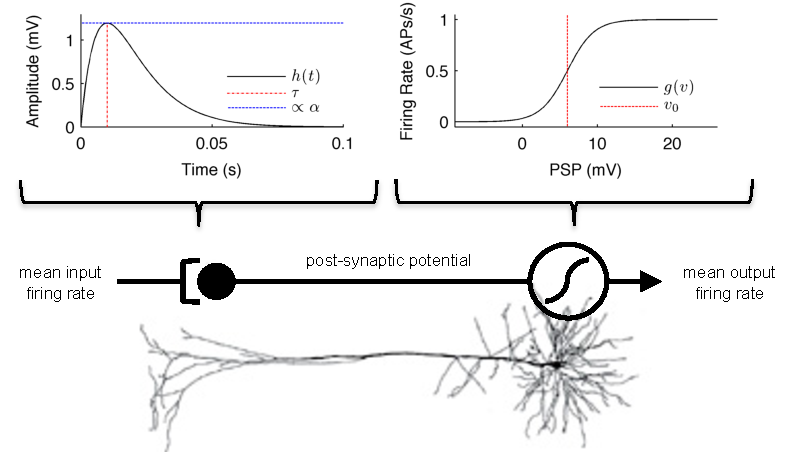
\includegraphics[scale=1]{./Figures/pdf/StandardNeuralMass.pdf}
	\caption{\textbf{Graphical Representation of the Neural Mass Model.} The neural mass model converts an input firing rate to a mean post-synaptic potential by a convolution with the post-synaptic response kernel. The membrane potential is converted to output firing rate by the sigmoidal activation function.} 

Since this model can be considered a statistical approximation to the actual brain dynamics we allow for model error and unmodelled inputs to be incorporated through the disturbance term $e_n(t)$ giving
\begin{align}
	\mathrm{d}\, v_n(t) =& z_n(t)\,\mathrm{d}t \\
	\mathrm{d}\, z_n(t) =& \alpha_{mn}\zeta_{mn} g_m(v_m(t)) - 2\zeta_{mn}z_n(t) - \zeta^2_{mn} v_n(t)\,\mathrm{d}t + \mathrm{d}\,w_n(t),
\end{align}
where $\zeta_{mn}$ is the reciprocal of the synaptic time constant and $w_n(t)$ is a Wiener process that is independent of $v_n(t)$ and $w_n(t) - w_n(0) \sim \mathcal{N}(0,t)$. Note that we have switched notation using Ito's notation.


	\label{fig:StandardNeuralMass}
\end{figure}

\section{Discretisation}
Next we need a discrete time version of the neural mass model in order to be able to apply the estimation methods. Let the time step be denoted by $\delta t$. The discretisation is performed using the Euler-Maruyama method by
\begin{align}
	v_n(t+\delta t) = & z_n(t)\,\delta t + v_n(t) \\
	z_n(t+\delta t) =& \left(\alpha_{mn}\zeta_{mn} g_m(v_m(t)) - 2\zeta_{mn}z_n(t) - \zeta^2_{mn} v_n(t)\right)\,\delta t + z_n(t) + e_n(t),
\end{align}
where $e_n(t) = w_n(t + \delta t) - w_n(t) \sim \mathcal{N}(0,\delta t \,\sigma_n^2)$.

\section{Jansen and Rit}
An example of the model of a cortical column is shown in Figure~\ref{fig:JansenAndRit}.
\begin{figure}[ht]
	\centering
		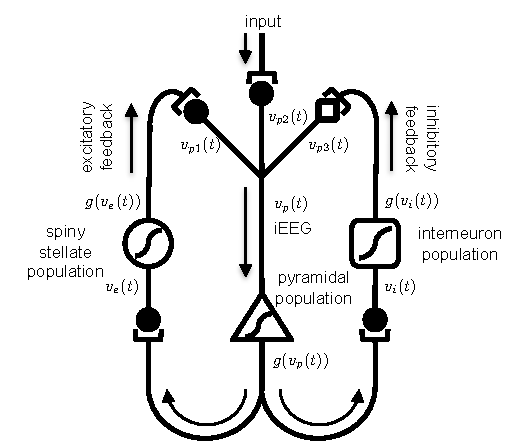
\includegraphics[scale=1]{./Figures/pdf/JansenAndRit.pdf}
	\caption{\textbf{Model of a Cortical Column.} The model shows three interconnected neural masses, which are pyramidal neurons, excitatory spiny stellate cells, and inhibitory interneurons. The specific subtype of neural population is defined by the parameters that describe the post-synaptic response kernels.}
	\label{fig:JansenAndRit}
\end{figure}

\begin{align}
	\mathrm{d}\,v_e(t) &= z_e(t)\,\mathrm{d}t \\
	\mathrm{d}\,z_e(t) &= (\alpha_{pe}\zeta_{pe}g\left(v_p(t)\right) - 2\zeta_{pe}z_e(t) - \zeta_{pe}^2v_e(t))\,\mathrm{d}t + \mathrm{d}\,w_e(t) \\
	\mathrm{d}\,v_i(t) &= z_i(t)\,\mathrm{d}t \\
	\mathrm{d}\,z_i(t) &= \left(\alpha_{pi}\zeta_{pi}g\left(v_p(t)\right) - 2\zeta_{e}z_i(t) - \zeta_{e}^2v_i(t)\right)\,\mathrm{d}t + \mathrm{d}\,w_i(t)\\
	\mathrm{d}\,v_{p1}(t) &= z_{p1}(t)\,\mathrm{d}t \\
	\mathrm{d}\,z_{p1}(t) &= (\alpha_{ep}\zeta_{ep}g\left(v_e(t)\right) - 2\zeta_{e}z_{p1}(t) - \zeta_{e}^2v_{p1}(t))\,\mathrm{d}t + \mathrm{d}\, w_{p1}(t)\\
	\mathrm{d}\,v_{p2}(t) &= z_{p2}(t)\,\mathrm{d}t \\
	\mathrm{d}\,z_{p2}(t) &= (\alpha_{ip}\zeta_{ip}g\left(v_i(t)\right) - 2\zeta_{i}z_{p2}(t) - \zeta_{i}^2v_{p2}(t))\,\mathrm{d}t  + \mathrm{d}\, w_{p2}(t) \\
	\mathrm{d}\,v_{p3}(t) &= z_{p3}(t)\,\mathrm{d}t \\
	\mathrm{d}\,z_{p3}(t) &= (\alpha_{xp}\zeta_{xp}\mu_x - 2\zeta_{e}z_{p3}(t) - \zeta_{e}^2v_{p3}(t))\,\mathrm{d}t + \mathrm{d}\,\alpha_{xp}w_x(t).
\end{align}

\begin{align}
	v_e(t+\delta t) &= z_e(t)\,\delta t + v_e(t)\\
	z_e(t+\delta t) &= (\alpha_{pe}g\left(v_p(t)\right) - 2\zeta_{e}z_e(t) - \zeta_{e}^2v_e(t))\,\delta t + z_e(t) + \varepsilon_e(t) \\
	v_i(t+\delta t) &= z_i(t)\,\delta t + v_i(t)\\
	z_i(t+\delta t) &= \left(\alpha_{pi}g\left(v_p(t)\right) - 2\zeta_{e}z_i(t) - \zeta_{e}^2v_i(t)\right)\,\delta t + z_i(t) + \varepsilon_i(t)\\
	v_{p1}(t+\delta t) &= z_{p1}(t)\,\delta t + v_{p1}(t) \\
	z_{p1}(t+\delta t) &= (\alpha_{ep}g\left(v_e(t)\right) - 2\zeta_{e}z_{p1}(t) - \zeta_{e}^2v_{p1}(t))\,\delta t + z_{p1}(t) + \varepsilon_{p1}(t)\\
	v_{p2}(t+\delta t) &= z_{p2}(t)\,\delta t + v_{p2}(t) \\
	z_{p2}(t+\delta t) &= (\alpha_{ip}g\left(v_i(t)\right) - 2\zeta_{i}z_{p2}(t) - \zeta_{i}^2v_{p2}(t))\,\delta t + z_{p2}(t) + \varepsilon_{p2}(t) \\
	v_{p3}(t+\delta t) &= z_{p3}(t)\,\delta t + v_{p3}(t) \\
	z_{p3}(t+\delta t) &= (\alpha_{xp}\mu_x - 2\zeta_{e}z_{p3}(t) - \zeta_{e}^2v_{p3}(t))\,\delta t + z_{p3}(t) + \varepsilon_x(t).
\end{align}

\bibliographystyle{plain}
\bibliography{}
\end{document}
